\documentclass{beamer}
%Для защит онлайн лучше использовать разрешение 16x9
%\documentclass[aspectratio=169]{beamer}

\usepackage{beamerthemesplit}
\usepackage{wrapfig}
\usetheme{SPbGU}
\usepackage{pdfpages}
\usepackage{amsmath}
\usepackage{cmap} 
\usepackage[T2A]{fontenc} 
\usepackage[utf8]{inputenc}
\usepackage[english,russian]{babel}
\usepackage{indentfirst}
\usepackage{amsmath}
\usepackage{tikz}
\usepackage{multirow}
\usepackage[noend]{algpseudocode}
\usepackage{algorithm}
\usepackage{algorithmicx}
\usetikzlibrary{shapes,arrows}
\usepackage{fancyvrb}
\usepackage{appendixnumberbeamer}

\newtheorem{rutheorem}{Теорема}
\newtheorem{ruproof}{Доказательство}
\newtheorem{rudefinition}{Определение}
\newtheorem{rulemma}{Лемма}

\beamertemplatenavigationsymbolsempty

% То, что в квадратных скобках, отображается внизу по центру каждого слайда. 
\title[Параллелизация miniKanren]{Параллелизация conde в урезанной реализации miniKanren для OCaml}

% То, что в квадратных скобках, отображается в левом нижнем углу. 
\institute[СПбГУ]{}

% То, что в квадратных скобках, отображается в левом нижнем углу.
\author[Андрей Диденко]{Андрей Антонович Диденко, 241 группа}
 
\begin{document}
{
\setbeamertemplate{footline}{}
% Лого университета или организации, отображается в шапке титульного листа
\begin{frame}
  
\includegraphics[width=1.4cm]{pictures/SPbGU_Logo.png}
  \vspace{-35pt}
  \hspace{-10pt}
  \begin{center}
    \begin{tabular}{c}
      \scriptsize{Санкт-Петербургский государственный университет} \\
      \scriptsize{Кафедра системного программирования}
    \end{tabular}
    \titlepage
  \end{center}

  \btVFill

  {\scriptsize
    % У научного руководителя должна быть указана научная степень
    {\bfseries Научный руководитель:} Д.С.Косарев, ассистент кафедры системного программирования \\
    % Консультанта может и не быть. Должна быть указана должность или ученая степень
    % {\bfseries Консультант:}  к.ф.-м.н. Д.С.Косарев, "MatMex, JetBrains Research laboratory" \\
    % Для курсовой не обязателен. Должна быть указана должность или ученая степень
    % {\bfseries Рецензент:} д.т.н., проф. И.И. Иванов, исполнительный директор ООО ``Рога и копыта''
  }
  \begin{center}
    \vspace{5pt}
    \scriptsize{Санкт-Петербург\\
      2022}
  \end{center}

\end{frame}
}

\begin{frame}[fragile]
  \frametitle{Введение}
  \begin{itemize}
    \item Работа направлена на повышение эффективности вычислений на языке miniKanren путем декомпозиции задачи на потоках
          % Краткий обзор тематики работы (как вариант --- устно, пока показывается титульный слайд)
    \item Данное решение предназначено для разработчиков, ипользующих miniKanren
          % Не нужно определять общеизвестные понятия
    \item Сообщество minikanren всерьез еще этим не занималось, поэтому у работы нет аналогов
          % Применимость/полезность данной работы, обоснование выбора именно этой темы
          % \item Если тема похожа на темы других работ (в том числе прошлых лет), надо явно описать разницу
  \end{itemize}
\end{frame}

\begin{frame}
  \frametitle{Используемые инструменты, подходы}
  \begin{itemize}
    \item За основу взят язык программирования OCaml, а также встаиваемый в него язык miniKanren
    \item Для разработки моего проекта была задействована библиотека Domainslib для Ocaml версии 5
    \item В 5 версии добавлены инструменты для параллелизации с более удобным функционалом
  \end{itemize}

\end{frame}

% \begin{frame}
%   \frametitle{Существующие решения}
%   Возможно, предметная область сложна и потребуется больше одного слайда, но затягивать введение не стоит. Постарайтесь уложиться в 1--2 слайда
%   \begin{itemize}
%     \item Выводы
%           \begin{itemize}
%             \item Подвести итог
%             \item Указать недостатки существующих подходов, на борьбу с которыми
%                   направленна данная работа
%             \item Чётко сформулировать существующую проблему, которая будет решаться в данной работе
%           \end{itemize}
%   \end{itemize}
% \end{frame}


% Обязательный слайд: четкая формулировка цели данной работы и постановка задачи
% Описание выносимых на защиту результатов, процесса или особенностей их достижения и т.д.
\begin{frame}
  \frametitle{Постановка задачи}
  \textbf{Целью} работы является распараллеливание miniKanren %озвученной выше  

  \textbf{Задачи}:
  \begin{itemize}
    % \item Выбрать алгоритм, подход, метод %основываясь на проведённом анализе проблемы, области, существующих решений
    \item Научиться параллелить две независимые задачи на miniKanren
          % \item Доказать корректность алгоритма
    \item Реализовать предложенный алгоритм
    \item Провести экспериментальное исследование предложенной реализации
  \end{itemize}
\end{frame}

%Идеально, если есть по одному слайду на каждую поставленную задачу            

\begin{frame}
  \frametitle{Алгоритм распараллеливания}
  \begin{itemize}
    \item 1.Рассматривая реализацию миниканрен на окамл,которая называется unicanren,
          придём к выводу, что можно распараллелить функцию Conde.
    \item При попытке параллелить функцию eval, результаты оказались отрицательным
    \item Делаем вывод,что необходимо параллелить run. Хотим доставать ответы по мере поступаления изнутри функции и вытягивать их на верхний уровень(в ответ)
  \end{itemize}
\end{frame}


\begin{frame}[fragile]
  \frametitle{Новый алгоритм\footnote{Иллюстративные возможности: таблицы, картинки, код}}
  % Задается ширина столбцов
  \begin{tabular}{p{5cm} p{7cm}}
    % Фрагмент кода
    \begin{minipage}{3in}
      \begin{Verbatim}[commandchars=\\\{\}]

        \textcolor{blue}{string} res = \textcolor{orange}{""};
        \textcolor{blue}{for}(i = 0; i < l; i++) \{
        res = \textcolor{orange}{"()"} + res;
        \}

      \end{Verbatim}
    \end{minipage}
                &
    Результат (SPPF):
    \\
    Аппроксимация:
                &
    % Картинка. Изображения должны быть векторными. Исключения --- снимки экрана.
    \multirow{-2}*{\!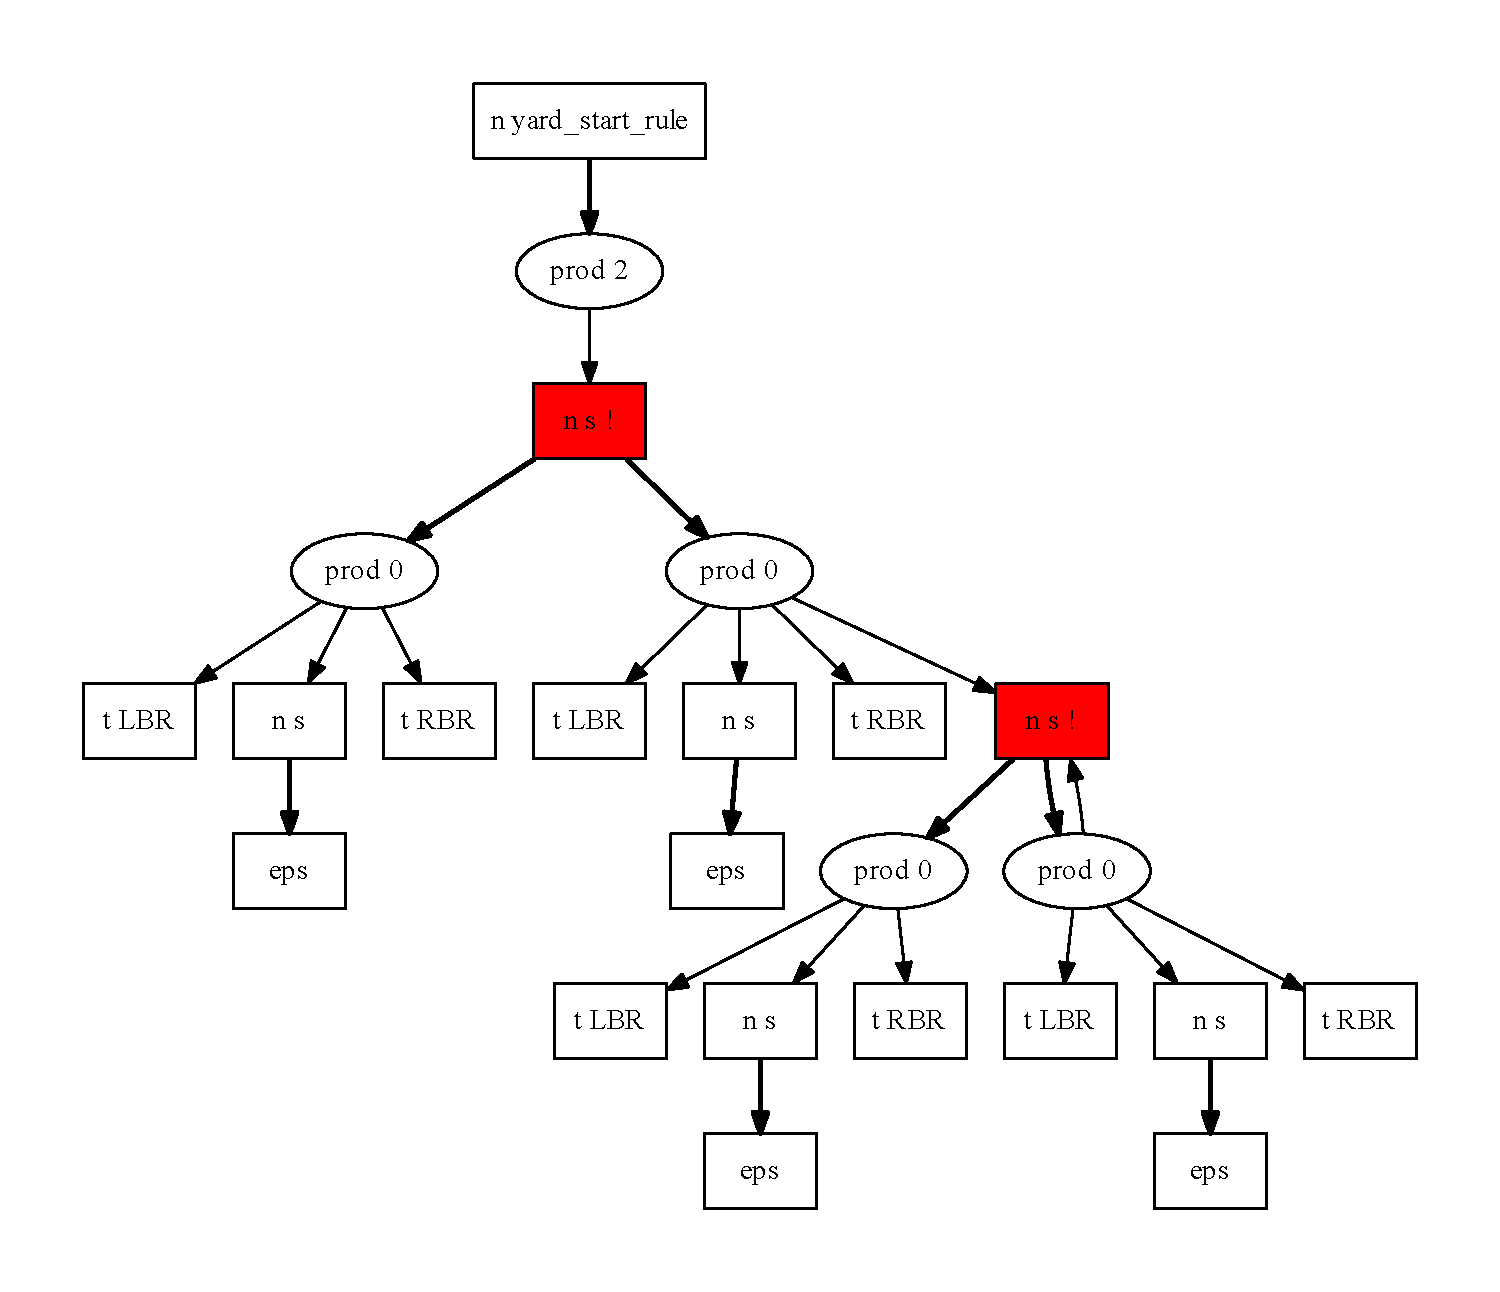
\includegraphics[width=6.8cm]{pictures/out3.pdf}}
    \\
    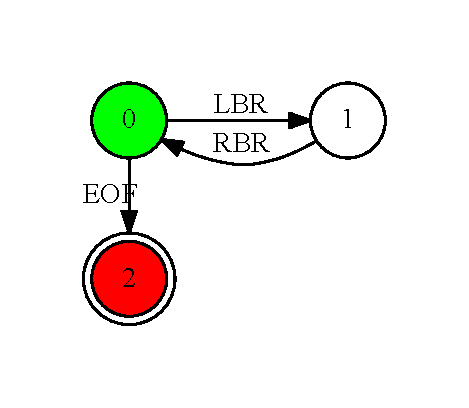
\includegraphics[width=2.5cm]{pictures/in3.pdf}
                &
    \\
    Грамматика: &
    \\
    \vspace{-20pt}
    % Можно формулы писать
    $$
      \begin{array}{crcl}
         & start & ::= & s                                              \\
         & s     & ::= & \mbox{\texttt{LBR }} s \mbox{\texttt{ RBR }} s \\
         & s     & ::= & \epsilon
      \end{array}
    $$
                &
  \end{tabular}
\end{frame}


\begin{frame}[fragile]
  \frametitle{Доказательство корректности алгоритма}
  {\tiny Формулировки утверждений. Идеи доказательств проговариваются устно.}
  \begin{rutheorem}[Пифагора: геометрическая формулировка]
    В прямоугольном треугольнике площадь квадрата, построенного на гипотенузе, равна сумме площадей квадратов, построенных на катетах.
  \end{rutheorem}

  \begin{rutheorem}[Пифагора: алгебраическая формулировка]
    В прямоугольном треугольнике квадрат длины гипотенузы равен сумме квадратов длин катетов.

    То есть, если обозначить длину гипотенузы треугольника через $c$, а длины катетов
    через $a$ и $b$, получим верное равенство: $a^2 + b^2 = c^2$.
  \end{rutheorem}

  \begin{rutheorem}[Обратная теорема Пифагора]
    Для всякой тройки положительных чисел a, b и c, такой, что $a^2 + b^2 = c^2$, существует прямоугольный треугольник с катетами a и b и гипотенузой c.
  \end{rutheorem}
\end{frame}

\begin{frame}[fragile]
  \frametitle{Архитектура решения}
  \begin{itemize}
    \item В реализации интересны архитектура, библиотеки, инструменты
    \item Не надо добавлять на слайд примеры кода
  \end{itemize}
  \begin{center}
    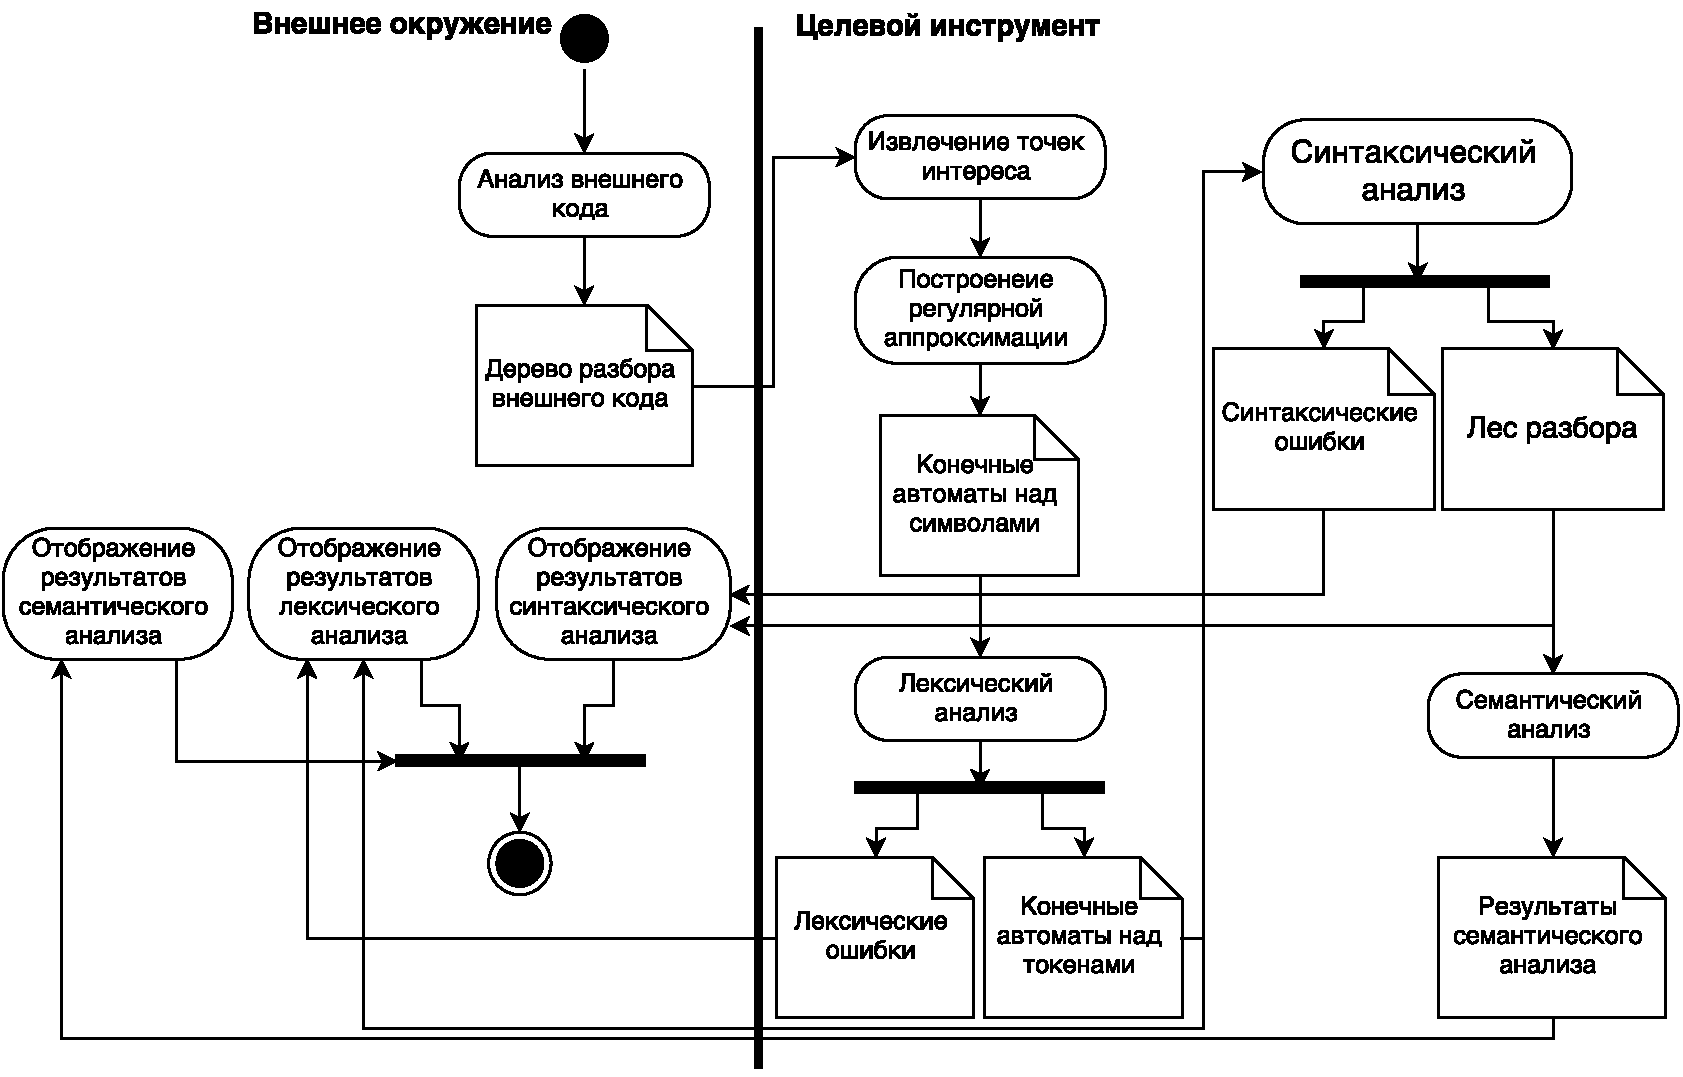
\includegraphics[width=0.8\textwidth]{pictures/Activ_SEL_Processing.pdf}
  \end{center}
\end{frame}

\begin{frame}[t]
  \frametitle{Экспериментальное исследование}
  Постановка эксперимента
  \begin{itemize}
    \item На каком наборе данных проводилось экспериментальное исследование, почему были выбраны именно эти данные
    \item На каком оборудовании проводилось исследование
    \item Какие решения были выбраны для сравнения и почему
  \end{itemize}
\end{frame}

\begin{frame}[t]
  \frametitle{Результаты экспериментального исследования}
  \begin{itemize}
    \item Какие результаты показало экспериментальное исследование
    \item Желательно привести графики, иллюстрирующие полученные результаты
          \begin{itemize}
            \item У иллюстраций должны быть подписи, у графиков --- легенда, подписи к осям, например:
          \end{itemize}
  \end{itemize}
  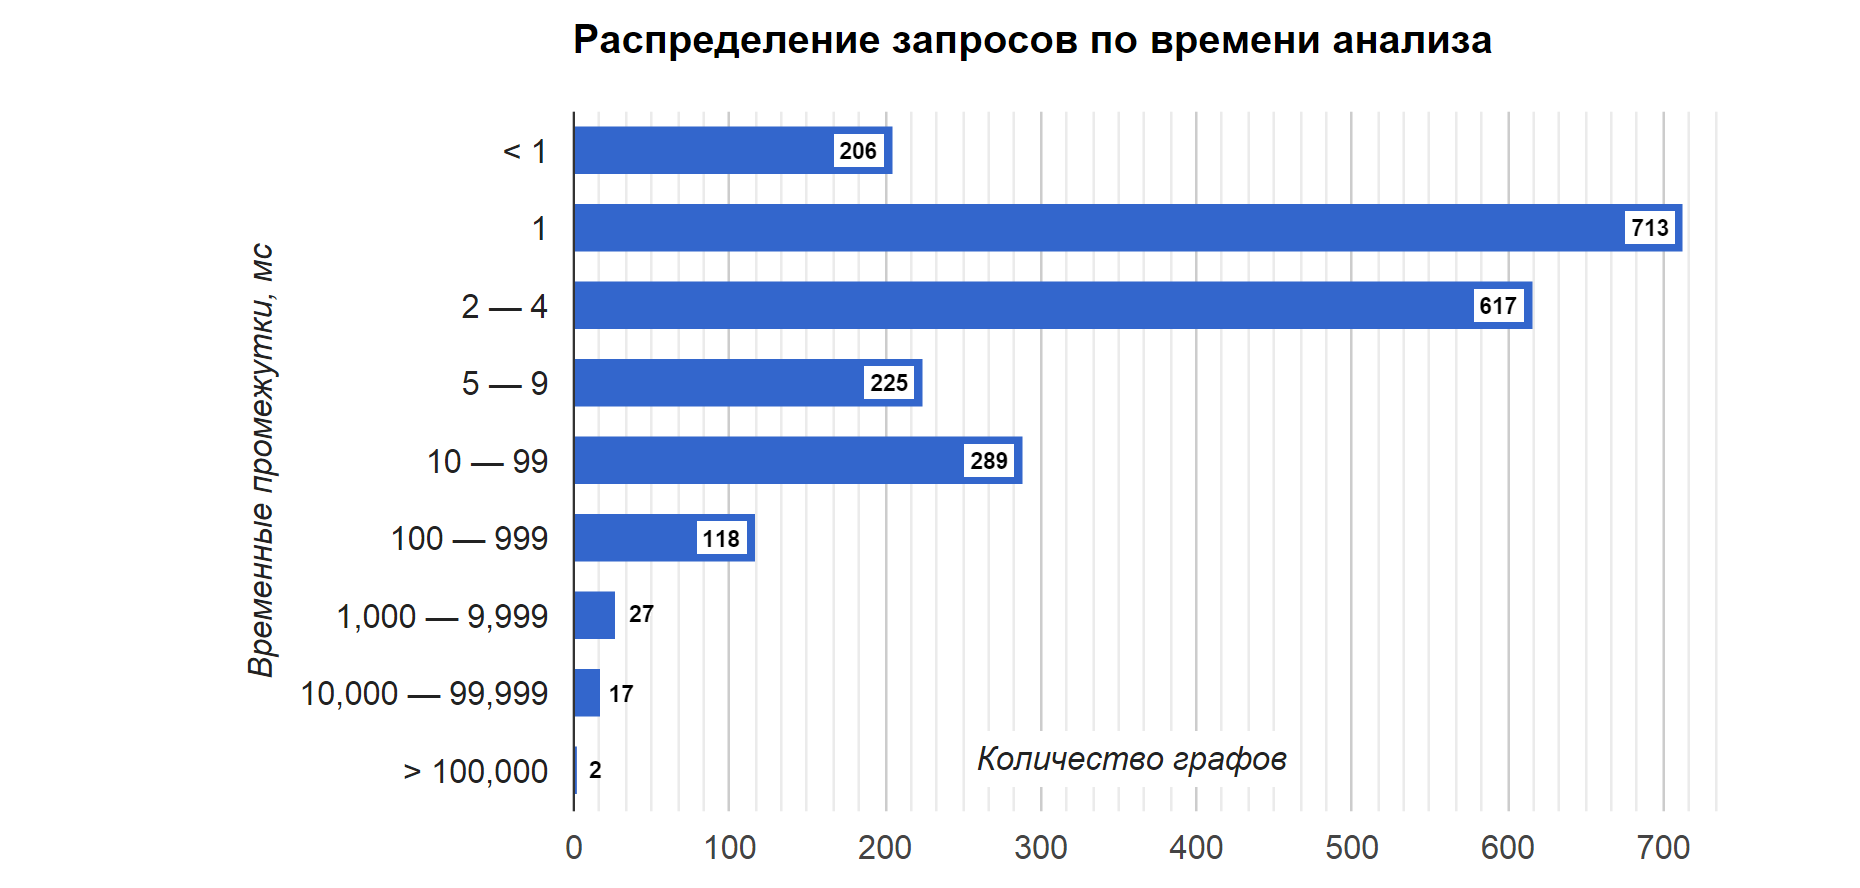
\includegraphics[width=10cm]{pictures/dist.png}
\end{frame}


\begin{frame}
  \frametitle{Результаты}
  \begin{itemize}
    \item Практически то же, что и на слайде с постановкой задачи, но в совершенной форме --- что делал лично автор
    \item Четкое отделение результатов своей работы (особенно для коллективных работ)
    \item Формулировать глаголами совершенного вида в прошедшем времени (``сделано'', ``получено'')
    \item Обсуждение (ограничения, валидность, альтернативы)
    \item Не нужно слайдов типа ``Все'', ``Вопросы?'', ``Спасибо за внимание''
  \end{itemize}

  \begin{itemize}
    \item Если результаты были представлены на конференции и опубликованы, это желательно указать
  \end{itemize}
\end{frame}

%\addtocounter{framenumber}{1}
\appendix


\end{document}